\chapter{Specific Requirements}
This section is devoted to a specific description of every kind of requirement the
system has to deal with in order to achieve all the functionalities described.
\section{External interface Requirements}
\subsection{User Interfaces}
The mobile app is the interface which permit customers to enjoy CLup services. Whether installed on a smartphone or on a ticketing kiosk, it is the only way
for a customer to use CLup.
User interface mockups of most important pages of the app are shown below.

\vspace{0.5cm}
\begin{minipage}{.5\textwidth}
	\centering
	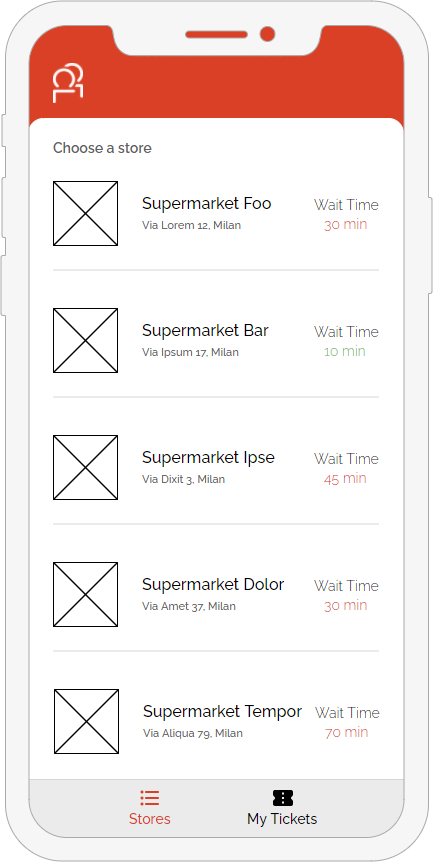
\includegraphics[scale=0.8]{home}
	\captionsetup{type=figure}
	\caption{App home.}
\end{minipage}%
\begin{minipage}{.5\textwidth}
	\centering
	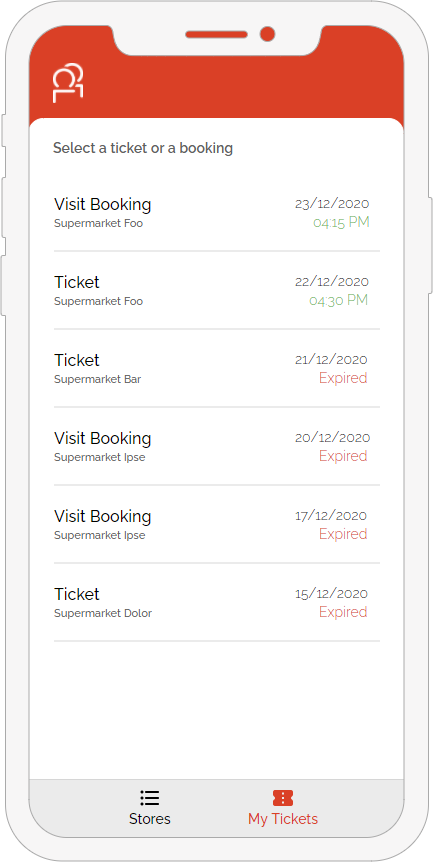
\includegraphics[scale=0.8]{my_tickets}
	\captionsetup{type=figure}
	\caption{Tickets list.}
\end{minipage}

\clearpage

\begin{minipage}{.5\textwidth}
	\centering
	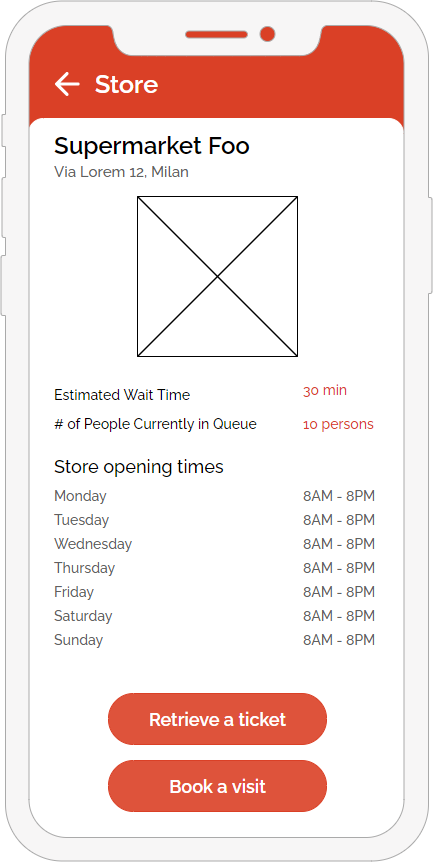
\includegraphics[scale=0.8]{store}
	\captionsetup{type=figure}
	\caption{Store page.}
\end{minipage}%
\begin{minipage}{.5\textwidth}
	\centering
	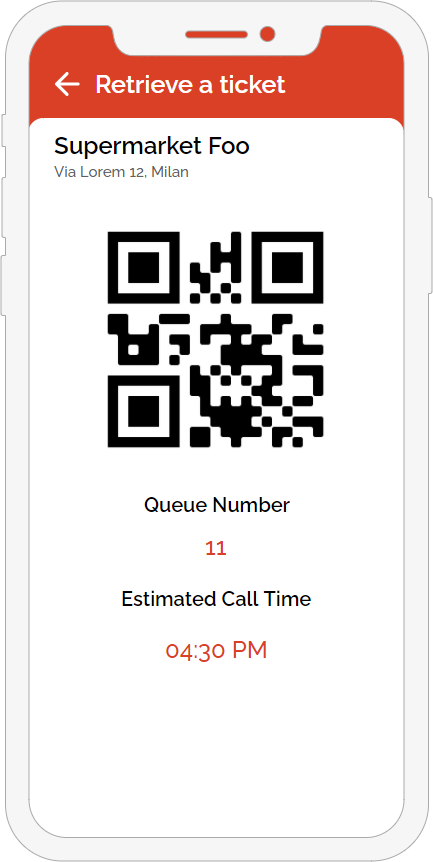
\includegraphics[scale=0.8]{ticket}
	\captionsetup{type=figure}
	\caption{Ticket Retrieved.}
\end{minipage}

\vspace{1cm}

\begin{minipage}{.5\textwidth}
	\centering
	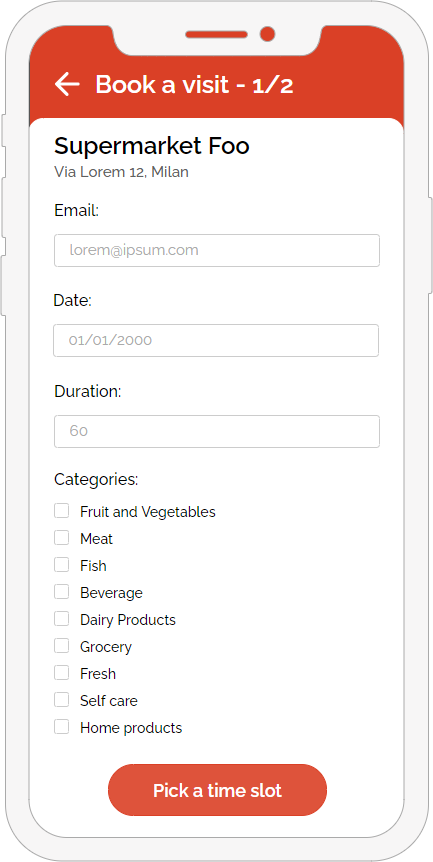
\includegraphics[scale=0.8]{book1}
	\captionsetup{type=figure}
	\caption{Book a visit (1/2).}
\end{minipage}%
\begin{minipage}{.5\textwidth}
	\centering
	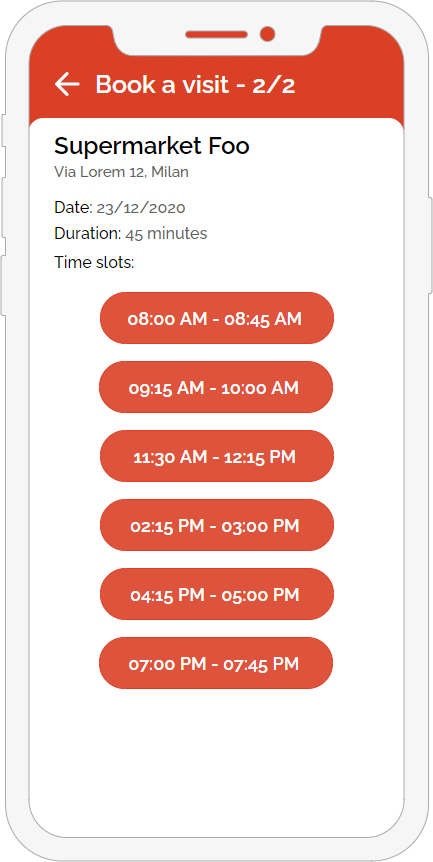
\includegraphics[scale=0.8]{book2}
	\captionsetup{type=figure}
	\caption{Book a visit (2/2).}
\end{minipage}

\vspace{1cm}

\begin{figure}[H]
	\centering
	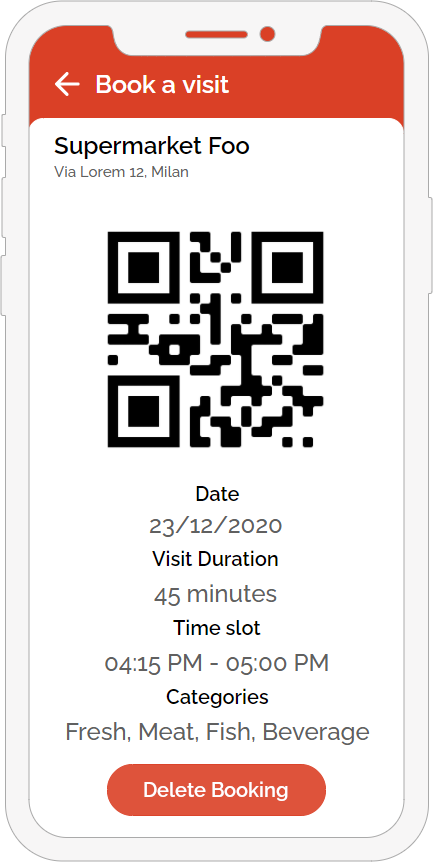
\includegraphics[scale=0.8]{book3}
	\caption{Visit booked.}
\end{figure}

\clearpage

Store managers and store employees use a web based interface for enjoying CLup features. The CLup admins can login at the same interface as well.
User interface mockups of most important pages of the web dashboard are shown below.
\vspace{0.5cm}
\begin{figure}[H]
	\centering
	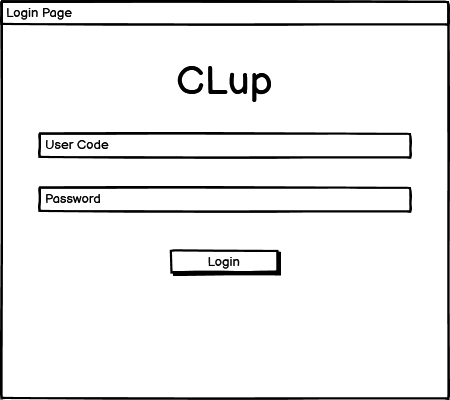
\includegraphics[width=0.64\linewidth]{login}
	\caption{Dashboard login.}
\end{figure}
\begin{figure}[H]
	\centering
	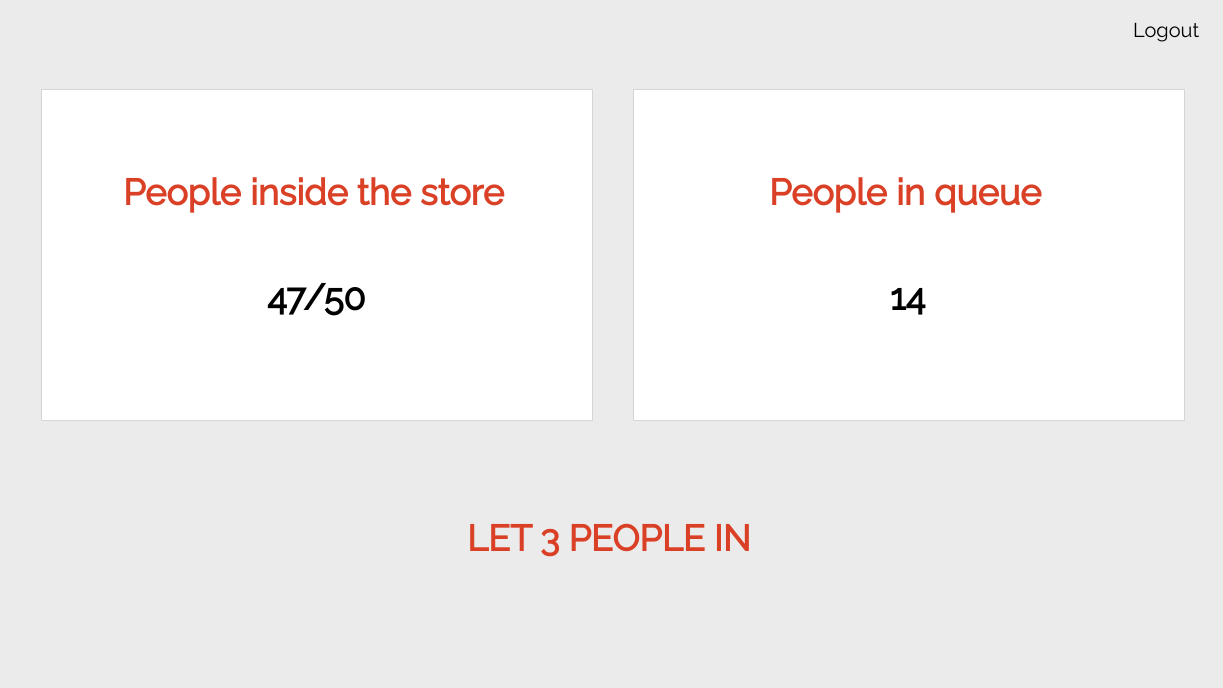
\includegraphics[width=0.64\linewidth]{employee}
	\caption{Employee homepage.}
\end{figure}
\begin{figure}[H]
	\centering
	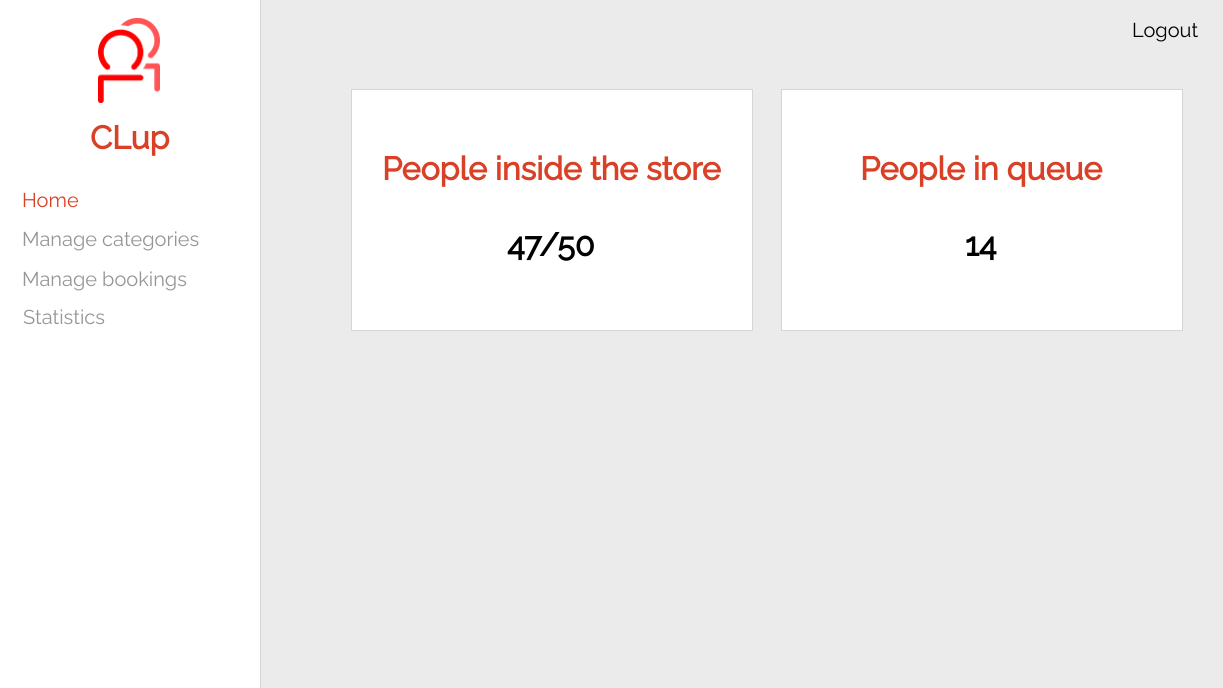
\includegraphics[width=0.64\linewidth]{dashboard1}
	\caption{Manager homepage.}
\end{figure}
\begin{figure}[H]
	\centering
	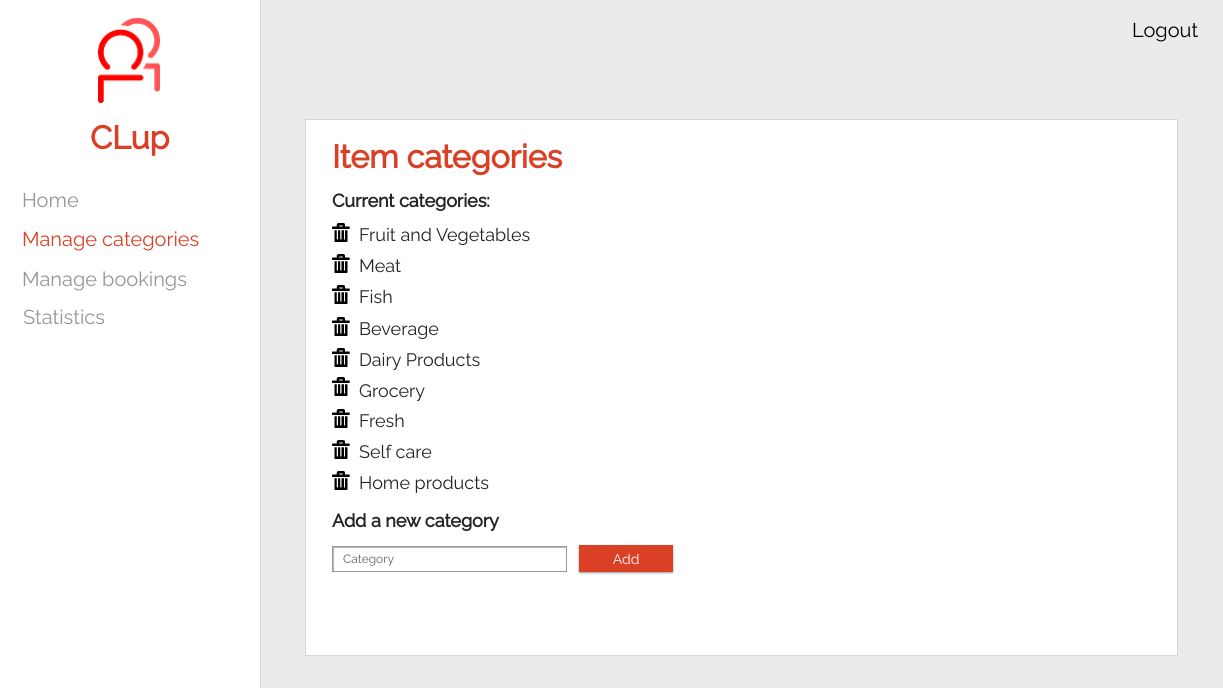
\includegraphics[width=0.64\linewidth]{dashboard2}
	\caption{Item categories page.}
\end{figure}
\begin{figure}[H]
	\centering
	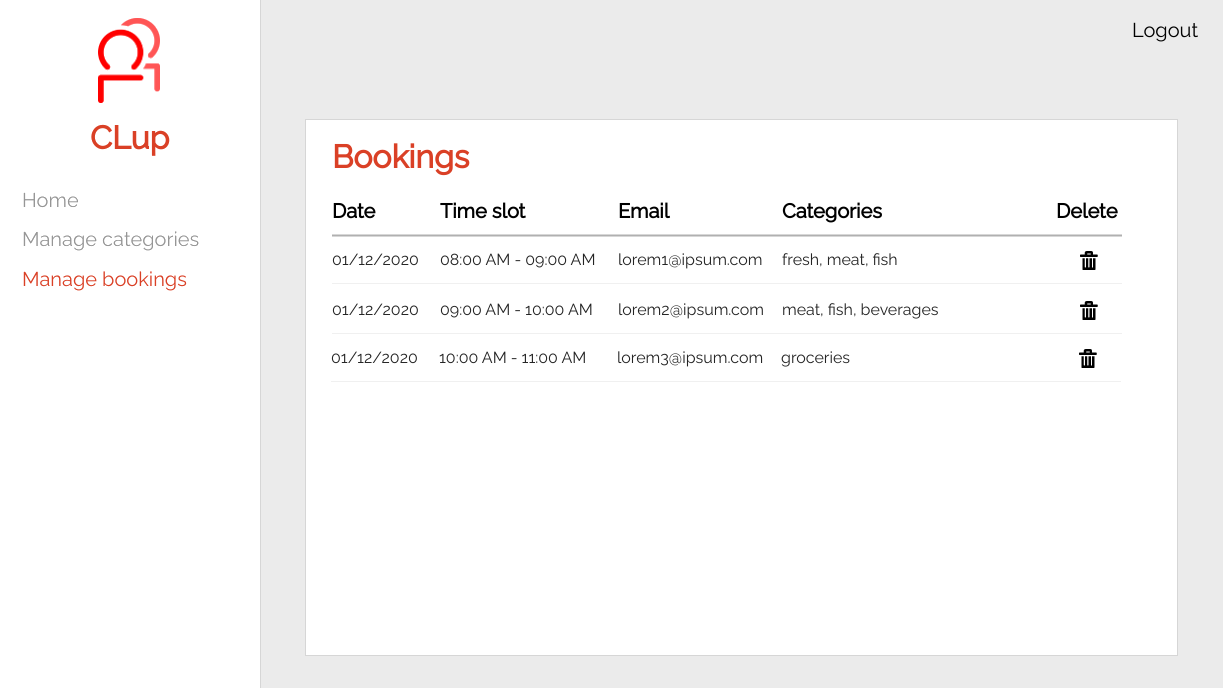
\includegraphics[width=0.64\linewidth]{dashboard3}
	\caption{Bookings list page.}
\end{figure}
\begin{figure}[H]
	\centering
	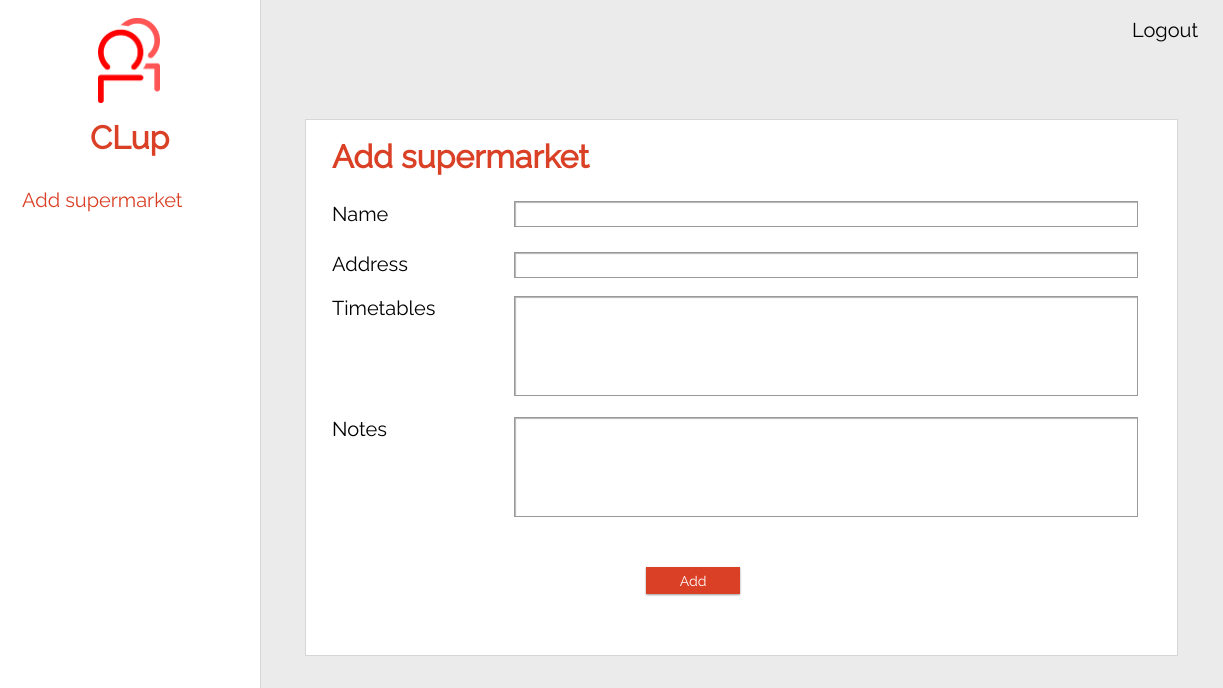
\includegraphics[width=0.64\linewidth]{new_store}
	\caption{Admin new supermarket page.}
\end{figure}

\clearpage

\subsection{Hardware Interfaces}
In addition to interfacing with computers (via a web browser), Clup interfaces with smartphones and their GPS module.
\subsection{Software Interfaces}
The system interfaces with a external map API for computing the distance between current place and store. It also permit to receive data
about QR codes via the public API.
\subsection{Communication Interfaces}
All the communications from and to CLup are made via HTTPS.

\section{Functional Requirements}
In this section, it is given a complete description of the functional requirements of the system.

    \subsection{Requirements}
    \subsubsection{Customer}
        \begin{enumerate}[series=requirements, label=\textbf{R.\arabic*}, leftmargin=+.3in]
            \item \itemtext{req:custQueue}{The system shall allow customers to line-up remotely in a store queue.}
            \item \itemtext{req:custTicket}{The system shall generate a new ticket when a customer enters a queue.}
            \item \itemtext{req:custTicketKiosk}{The system shall allow customers which do not have a smartphone to get a ticket in place.}
            \item \itemtext{req:custNum}{The system shall allow customers to view the number of people lined up in a queue.}
            \item \itemtext{req:custTime}{The system shall give customers an estimated waiting time.}
            \item \itemtext{req:custGps}{The system shall retrieve the GPS position while the user is subscribed to a queue.}
            \item \itemtext{req:custLeave}{The system shall allow customers to leave a queue.}
            \item \itemtext{req:custFilter}{The system shall allow customers to filter stores by name.}
            \item \itemtext{req:custTtl}{The system shall notify customers when it's time to leave for the store.}
            \item \itemtext{req:custBook}{The system shall allow customers to book-a-visit to the store and send them the receipt via email.}
            \item \itemtext{req:custItems}{The system shall allow book-a-visit customers to specify the main categories of item they intend to buy.}
            \item \itemtext{req:custDelete}{The system shall allow customers to delete a booked visit.}
            \item \itemtext{req:custNotifyDelete}{The system shall notify customers when a ticket or booked visit is deleted.}
        \end{enumerate}

    \subsubsection{Store manager}
    \begin{enumerate}[resume*=requirements]
        \item \itemtext{req:mngLogin}{A registered store manager must be able to login to the system by using his/her credentials.}
        \item \itemtext{req:mngViewStore}{The system shall allow store managers to view the current status of people inside the store.}
        \item \itemtext{req:mngViewQueue}{The system shall allow store managers to view the current status of people in the queue.}
         \item \itemtext{req:mngViewBook}{The system shall allow store managers to view the booked visits to the store.}
        \item \itemtext{req:mngCapStore}{The system shall allow store managers to set a maximum cap of people inside the store.}
        \item \itemtext{req:mngCapQueue}{The system shall allow store managers to set a maximum cap of people in the queue.}
        \item \itemtext{req:mngDeleteTickets}{The system shall allow store managers to delete tickets and booked visits.}
    \end{enumerate}

    \subsubsection{Store staff}
    \begin{enumerate}[resume*=requirements]
        \item \itemtext{req:stfLogin}{A registered store staff must be able to login to the system by using his/her credentials.}
        \item \itemtext{req:stfViewStore}{The system shall allow store staff to view the current status of people inside the store.}
        \item \itemtext{req:stfViewQueue}{The system shall allow store staff to view the current status of people in the queue.}
    \end{enumerate}

    \subsubsection{CLup admin}
    \begin{enumerate}[resume*=requirements]
        \item \itemtext{req:admRegister}{The system shall allow CLup admins to register new supermarkets.}
        \item \itemtext{req:admCredentials}{The system shall generate new manager and staff credential for each supermarket registered.}
    \end{enumerate}

    \subsection{Goal mapping on requirements}

    \begin{description}     
        
        
        \item \printitem{goal:avoidQueue}
           		
        \begin{description}       	
   
        	\item \printitem{goal:custHazardSit}
        				
			\printitem{req:custQueue}			
			\printitem{req:custNum}					
			\printitem{req:custTime}			
			\printitem{req:custTtl}		
			\printitem{req:custBook}			
			\printitem{req:custItems}			
				
			\printitem{dom:smartphone}			
			\printitem{dom:categories}			
			\printitem{dom:custEmail}			
			\printitem{dom:oneToOneQr}			
			\printitem{dom:timeArrival}

		    		    
			\item \printitem{goal:storeHazardSit}
							
			\printitem{req:mngViewStore}
			\printitem{req:mngViewQueue}
			\printitem{req:mngViewBook}
			\printitem{req:mngCapStore}
			\printitem{req:mngCapQueue}
			\printitem{req:mngDeleteTickets}
			\printitem{req:stfViewStore}
			\printitem{req:stfViewQueue}
			
			\printitem{dom:categories}
			\printitem{dom:oneToOneQr}
			\printitem{dom:internetStores}
			\printitem{dom:employeeEntrance}
			\printitem{dom:timeArrival}
			\printitem{dom:capStores}
			

            \item \printitem{goal:shortenTime}   
                           
           	\printitem{req:custQueue}
           	\printitem{req:custNum}
           	\printitem{req:custTime}
           	\printitem{req:custTtl}
           	\printitem{req:custBook}
           	
           	\printitem{dom:smartphone}
           	\printitem{dom:workingGps}
           	\printitem{dom:gpsPrecision}
           	\printitem{dom:bringSmartphone}
           	\printitem{dom:employeeEntrance}
           	\printitem{dom:qrServiceReliable}
           	\printitem{dom:qrServiceApi}
           	\printitem{dom:timeArrival}


            \item \printitem{goal:arriveOnTime}                

           	\printitem{req:custQueue}
           	\printitem{req:custNum}
           	\printitem{req:custTime}
           	\printitem{req:custGps}
           	\printitem{req:custTtl}
           	\printitem{req:custBook}
           	
           	\printitem{dom:smartphone}
           	\printitem{dom:workingGps}
           	\printitem{dom:gpsPrecision}
           	\printitem{dom:bringSmartphone}
           	\printitem{dom:timeArrival}
		\end{description}

        \item \printitem{goal:otherTasks}

       	\printitem{req:custQueue}
       	\printitem{req:custNum}
       	\printitem{req:custTime}
       	\printitem{req:custTtl}
       	\printitem{req:custBook}
       	
       	\printitem{dom:smartphone}
       	\printitem{dom:workingGps}
       	\printitem{dom:gpsPrecision}
       	\printitem{dom:custEmail}
       	\printitem{dom:bringSmartphone}
       	\printitem{dom:timeArrival}


        \item \printitem{goal:easyExp}    
       	
       	\printitem{req:custTicket}
       	\printitem{req:custNum}
       	\printitem{req:custTime}
       	\printitem{req:custLeave}
       	\printitem{req:custFilter}
       	\printitem{req:custBook}
       	\printitem{req:custDelete}
       	\printitem{req:custNotifyDelete}
       	
       	\printitem{dom:smartphone}
       	\printitem{dom:workingGps}
       	\printitem{dom:uniqueName}
       	\printitem{dom:qrServiceReliable}
       	\printitem{dom:storeRegistered}
       	\printitem{dom:storeKiosk}


        \item \printitem{goal:enjoyService}
	
       	\printitem{req:custQueue}
       	\printitem{req:custTicketKiosk}
       	\printitem{req:custBook}
       	
       	\printitem{dom:smartphone}
       	\printitem{dom:internetStores}
       	\printitem{dom:storeRegistered}
       	\printitem{dom:storeKiosk}
    

        \item \printitem{goal:monitorAccess}  
             
       	\printitem{req:mngLogin}
       	\printitem{req:mngViewStore}
       	\printitem{req:mngViewQueue}
       	\printitem{req:mngViewBook}
       	\printitem{req:stfLogin}
       	\printitem{req:stfViewStore}
       	\printitem{req:stfViewQueue}
       	\printitem{req:admRegister}
       	\printitem{req:admCredentials}
       	
       	\printitem{dom:internetStores}
       	\printitem{dom:employeeEntrance}
       	\printitem{dom:storeRegistered}
       	\printitem{dom:capStores}


        \item \printitem{goal:knowInAdvance}
        
       	\printitem{req:mngViewStore}
       	\printitem{req:mngViewQueue}
       	\printitem{req:mngViewBook}
       	\printitem{req:stfViewStore}
       	\printitem{req:stfViewQueue}
       	
       	\printitem{dom:smartphone}
       	\printitem{dom:categories}
       	\printitem{dom:internetStores}
       	\printitem{dom:storeRegistered}


        \item \printitem{goal:limitNumber}
               	
       	\printitem{req:mngCapStore}
       	\printitem{req:mngCapQueue}
       	\printitem{req:mngDeleteTickets}
	
       	\printitem{dom:smartphone}
       	\printitem{dom:categories}
       	\printitem{dom:internetStores}
       	\printitem{dom:storeRegistered}
       	\printitem{dom:timeArrival}
       	\printitem{dom:capStores}
   
    \end{description}

    \subsection{Scenarios}

    \subsection{Use cases description}
    Use cases capture functional requirements of a system from the users' perspective.
	
	\begin{table}[H]
    	\centering
		\begin{tabular}{@{}p{0.25\linewidth}p{0.71\linewidth}@{}}
			\toprule
			\textbf{Name} & Lorem \\
			
			\midrule
			\textbf{ID} & \usecaseindex ~\\
			\midrule
			\textbf{Actors} & Ipsum \\
			\midrule
			\textbf{Entry conditions} & Ipsum \\
			\midrule
			\textbf{Flow of events} & Ipsum \\
			\midrule
			\textbf{Exit conditions} & Ipsum \\
			\midrule
			\textbf{Exceptions} & Ipsum \\		
			
			\bottomrule		
		\end{tabular}
		\caption{\textit{Lorem} use case description}
	\end{table}


	\begin{table}[H]
		\centering
		\begin{tabular}{@{}p{0.25\linewidth}p{0.71\linewidth}@{}}
			\toprule
			\textbf{Name} & Lorem \\
			
			\midrule
			\textbf{ID} & \usecaseindex ~\\
			\midrule
			\textbf{Actors} & Ipsum \\
			\midrule
			\textbf{Entry conditions} & Ipsum \\
			\midrule
			\textbf{Flow of events} & Ipsum \\
			\midrule
			\textbf{Exit conditions} & Ipsum \\
			\midrule
			\textbf{Exceptions} & Ipsum \\		
			
			\bottomrule		
		\end{tabular}
		\caption{\textit{Lorem} use case description}
	\end{table}

    \subsection{Traceability matrix}
    \begin{center}
        \begin{tabular}{@{}p{0.25\linewidth}cccc@{}}
            \toprule
            \textbf{Item} & \textbf{\ref{req:custQueue}} & \textbf{\ref{req:custTicket}}
            & \textbf{\ref{req:custTime}} & \textbf{\ref{req:custNum}}\\
            \midrule
            Lorem Ipsum & \cmark \\
            Dolor Sit & & & \cmark \\

            \bottomrule
        \end{tabular}
    \end{center}


\section{Performance Requirements}

\section{Design Constraints}

\section{Software System Attributes}